\section{Methodology}
\label{methodology}

\subsection*{Environment}
Open environments with shifting populations are the long-term motivation for this framework. Initial pilot experiments using the OpenWorld environment from Craftium \cite{malagoncraftium} confirmed that with a small population and a short horizon, agents rarely encountered one another, so the Hebbian co-activity signal $c_{ij}(t)$ rarely fired and bonds never accumulated. We hypothesise that meaningful Hebbian dynamics in open-world settings require both larger populations and longer horizons. We therefore study the mechanism in a small-population cooperative setting where its effects can be measured in isolation. We introduce \emph{WIRE} (Wired Inter-agent Reasoning Evaluation), a five-stage environment built on Luanti in which agents progress through tasks of increasing coordination demand: solo skill acquisition, joint resource acquisition, a partially observable switch puzzle that can only be solved through targeted communication, and cooperative combat culminating in a boss fight (see \autoref{fig:five_chambers_curriculum}). Each stage builds \emph{mechanism-level interdependence} into the environment itself, so that the value of persistent social bonds can be assessed without needing the population scale that open environments require. WIRE thus serves as a controlled environment for the Hebbian mechanism. A detailed discussion of the environment-selection considerations is provided in \autoref{sec:env_selection}.

\begin{figure*}[t]
    \centering
    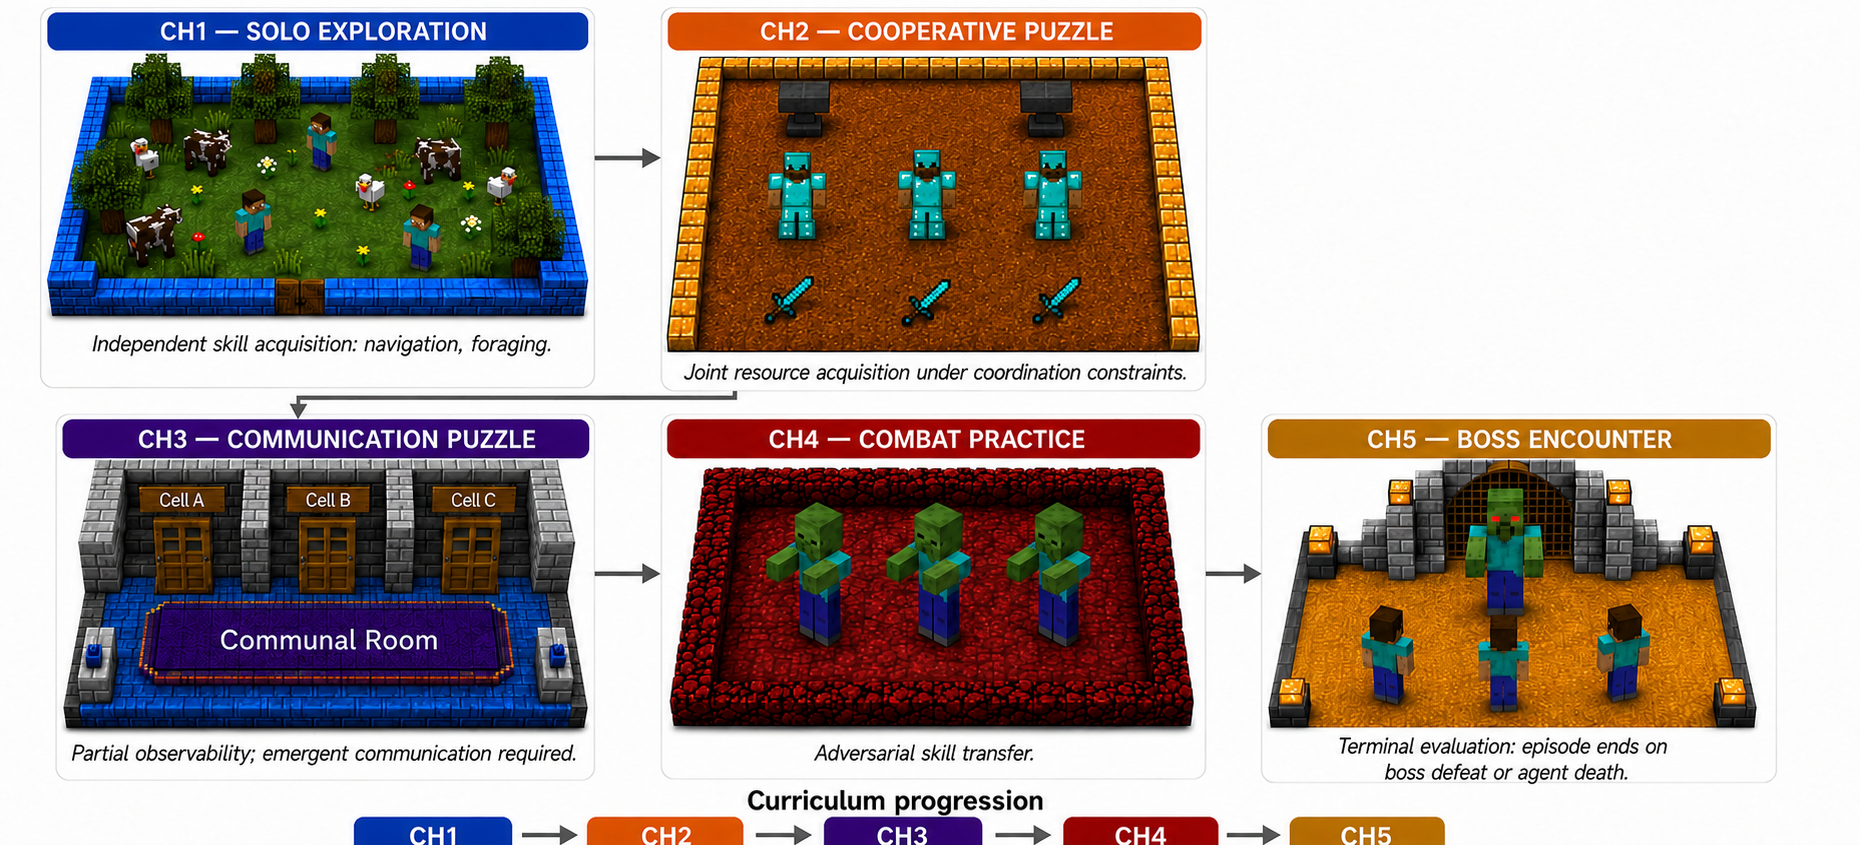
\includegraphics[width=\linewidth]{figures/env_minecraft.png}
    \caption{The WIRE environment (Wired Inter-agent Reasoning Evaluation). Agents progress through five chambers, each targeting a distinct coordination competency: solo skill acquisition (Ch1), cooperative resource acquisition under joint-action requirements (Ch2), targeted communication under partial observability (Ch3), team combat (Ch4), and a cooperative boss fight (Ch5). Episodes terminate on boss defeat or full team death.}
    \label{fig:five_chambers_curriculum}
\end{figure*}

\begin{figure*}[t]
\centering
\begin{tikzpicture}[
  font=\sffamily\footnotesize,
  >={Stealth[length=2.4mm,width=2mm]},
  soft/.style={blur shadow={shadow blur steps=6, shadow xshift=0pt, shadow yshift=-0.5mm, shadow opacity=22}},
  io/.style={draw=cEnv!75, line width=0.7pt, fill=cEnv!9, rounded corners=3pt, align=center,
             inner sep=4pt, minimum height=11mm, text width=19mm, soft},
  pill/.style={draw=cAgent!50, line width=0.5pt, fill=cAgent!10, rounded corners=4pt, align=center,
               font=\sffamily\scriptsize, inner sep=2pt, minimum height=6mm, text width=15mm},
  core/.style={draw=cCore!85, line width=1pt, fill=cCore!18, rounded corners=4pt, align=center,
               inner sep=4pt, minimum height=15mm, text width=24mm, soft},
  out/.style={draw=cCore!70, line width=0.6pt, fill=cCore!9, rounded corners=4pt, align=center,
              font=\sffamily\scriptsize, inner sep=3pt, minimum height=7mm, text width=24mm},
  rl/.style={draw=cRL!75, line width=0.8pt, fill=cRL!10, rounded corners=4pt, align=center,
             inner sep=4pt, minimum height=18mm, text width=41mm, soft},
  heb/.style={draw=cHeb!75, line width=0.8pt, fill=cHeb!9, rounded corners=4pt, align=center,
              inner sep=4pt, minimum height=18mm, text width=41mm, soft},
  title/.style={font=\sffamily\bfseries\footnotesize},
  arr/.style={-{Stealth[length=2.4mm,width=2mm]}, line width=0.8pt, rounded corners=2pt, draw=cEnv!85},
  flow/.style={-{Stealth[length=2.2mm]}, line width=0.7pt, dash pattern=on 2.2pt off 1.6pt, draw=cEnv!55},
  node distance=7mm and 9mm,
]

% ============ Tier 1: per-agent inference loop ============
% --- MindForge cognitive stack: 8 module pills in a 2x4 grid ---
\node[pill] (g1) {Perception};
\node[pill, right=2.5mm of g1] (g2) {Partner};
\node[pill, below=2.2mm of g1] (g3) {Interaction};
\node[pill, right=2.5mm of g3] (g4) {Task beliefs};
\node[pill, below=2.2mm of g3] (g5) {Episodic mem.};
\node[pill, right=2.5mm of g5] (g6) {Skills};
\node[pill, below=2.2mm of g5] (g7) {Auto-curric.};
\node[pill, right=2.5mm of g7] (g8) {Critic};
\begin{scope}[on background layer]
  \node[draw=cAgent!60, line width=0.8pt, fill=cAgent!4, rounded corners=5pt,
        fit=(g1)(g2)(g7)(g8), inner sep=3.2mm, inner ysep=5.5mm, soft] (stack) {};
\end{scope}
\node[title, text=cAgent!75, anchor=north] at ([yshift=-1.2mm]stack.north) {MindForge cognitive stack};

% --- environment + observation to the left of the stack ---
\node[io, left=9mm of stack] (obs) {Observation\\[1pt]$o_i^t$};
\node[io, left=of obs, fill=cEnv!13] (env) {Environment\\[1pt]\textbf{WIRE} (Luanti)};

% --- LLM core + outputs to the right of the stack ---
\node[core, right=9mm of stack] (llm) {\textbf{Frozen LLM}\\[1pt]Qwen3.5-2B\\[1pt]$+$ LoRA adapter};
\node[out, right=8mm of llm, yshift=4.5mm] (head) {action head $\phi \to a_i^t$};
\node[out, right=8mm of llm, yshift=-4.5mm, fill=cCore!5] (msg)  {message gen $\to m_i^t,\tau_i^t$};

% inference-path arrows
\draw[arr] (env) -- (obs);
\draw[arr] (obs) -- (stack);
\draw[arr] (stack) -- node[above, font=\sffamily\scriptsize, text=cEnv!70]{prompt} (llm);
\draw[arr] (llm.east) to[out=20,in=180] (head.west);
\draw[arr] (llm.east) to[out=-20,in=180] (msg.west);

% feedback arc: act in the environment
\draw[arr, draw=cCore!80]
  ([yshift=1mm]head.north) .. controls ($(head.north)+(0,13mm)$) and ($(env.north)+(0,15mm)$) ..
  node[above, font=\sffamily\scriptsize, text=black, pos=0.5]{act in environment: $a_i^t,\ m_i^t,\ \tau_i^t$}
  (env.north);

% ============ Tier 2: centralised training subsystems ============
\node[rl, below=22mm of stack, xshift=-6mm] (mappo)
  {centralised critic $V_\psi(s^t)$\\[2pt] advantage $A_i^t$ (GAE)\\[2pt] PPO clipped update};
\node[title, text=cRL!72, anchor=south] at ([yshift=1mm]mappo.north) {Reinforcement learning (MAPPO, CTDE)};

\node[heb, right=34mm of mappo] (hebb)
  {co-activity $c_{ij}(t)\;\cdot\;$ modulator $m_i(t)$\\[2pt] social graph $W(t)$\\[2pt] reward diffusion $r_i \!\to\! r_i'$};
\node[title, text=cHeb!75, anchor=south] at ([yshift=1mm]hebb.north) {Hebbian social plasticity};

% experience bus: environment -> both trainers (anchored in the gap, clear of the stack)
\coordinate (busY)   at ($(mappo.north)+(0,9mm)$);
\coordinate (busEnv) at (env.south |- busY);
\draw[flow] (env.south) -- (busEnv);
\draw[flow,-] (busEnv) -- (busEnv -| hebb.north);
\draw[flow] (busEnv -| mappo.north) -- (mappo.north)
      node[pos=0.45, right, font=\sffamily\scriptsize, text=cEnv!75]{$r_i^t,\,s^t$};
\draw[flow] (busEnv -| hebb.north) -- (hebb.north)
      node[pos=0.45, right, font=\sffamily\scriptsize, text=cEnv!75]{$r_i^t$, pos., comm.};

% couplings between the two trainers (wide gap keeps labels clear of boxes)
\draw[arr, draw=cRL!85] ([yshift=4mm]mappo.east) to[bend left=10]
      node[above, font=\sffamily\scriptsize, text=black]{$A_i^t$ (modulator)} ([yshift=4mm]hebb.west);
\draw[arr, draw=cHeb!85] ([yshift=-4mm]hebb.west) to[bend left=10]
      node[below, font=\sffamily\scriptsize, text=black]{$r_i'$ (diffused reward)} ([yshift=-4mm]mappo.east);

% policy update back up to the agent's LoRA adapter
\draw[arr, draw=cRL!85] ([xshift=8mm]mappo.north) to[out=80,in=-95]
      node[right, font=\sffamily\scriptsize, text=black, pos=0.62]{policy update (LoRA, $\phi$)} (llm.south);
\end{tikzpicture}
\caption{System overview. \textbf{Top --- per-agent inference loop.} Each agent's \emph{MindForge} cognitive stack turns the observation $o_i^t$ into an action-selection prompt; the frozen LLM with a LoRA adapter emits a discrete action $a_i^t$ (via the action head $\phi$) and, in a separate call, a targeted message $(m_i^t,\tau_i^t)$, both enacted in the WIRE environment. \textbf{Bottom --- centralised training.} MAPPO updates the LoRA adapter and action head from rollouts under centralised training with decentralised execution, while the Hebbian module maintains the reward-modulated social graph $W(t)$. The subsystems are coupled: the per-step advantage $A_i^t$ drives the Hebbian modulator, and reward diffusion redistributes rewards along $W(t)$ to produce the diffused reward $r_i'$ that enters the policy gradient.}
\label{fig:system_overview}
\end{figure*}

\subsection{Agent architecture}
\label{sec:agent_architecture}

An overview of the full system---the per-agent cognitive stack, the MAPPO reinforcement-learning layer, and the Hebbian social module that couples them---is shown in \autoref{fig:system_overview}. Each agent in WIRE is built on the \emph{MindForge} cognitive stack \cite{licua2025mindforge}: a frozen language model (Qwen3.5-2B throughout) serving as the per-agent reasoning core, augmented with cognitive modules that maintain the agent's situated understanding of the task, its teammates, and its own progress. When the reinforcement-learning layer is enabled, a low-rank adapter (LoRA) \cite{hu2022lora} is inserted into the attention layers and trained against environment reward; the rest of the model remains frozen. At each step, an agent receives a $320 \times 180$ first-person frame, a structured text context, and any messages addressed to it by teammates, and emits one discrete action together with an optional natural-language message addressed to one specific teammate.

\paragraph{Cognitive modules.}
Six modules feed into the action-selection prompt: \emph{perception beliefs} describe what the agent sees in action-relative spatial terms and flag unenacted action--target combinations as intrinsic-motivation targets \cite{georgeon2012interactional}; \emph{partner beliefs} maintain one entry per teammate summarising their chamber, gear, commitments, and reported schemes; \emph{interaction beliefs} extract actionable shared information like role assignments, switch and door status, combat coordination, team-level warnings from recent conversation; \emph{task beliefs} provide a procedural context for the current task, framed as a scheme that pairs an intended action with the observation the agent expects to see; \emph{episodic memory}, a ChromaDB vector store keyed on task embeddings, retrieves past attempts with a 70/30 success-to-failure ratio so the agent sees mostly positive examples without losing failure signal; and \emph{skills} stores successful action-thought pairs in a separate vector store for retrieval on similar tasks.

\paragraph{Auto-curriculum and critic.}
An auto-curriculum module proposes the next concrete task at every step, conditioned on the agent's current chamber, fired milestones, inventory, and a brief question-answer pass. Validity filters reject proposals that reference fixtures outside the agent's current chamber or that contain no actionable keyword, replacing them with a chamber-appropriate fallback. A critic module evaluates task success every twenty steps from the frame, last action, reward, status, inventory, and current task. The verdict drives three downstream effects: successful tasks promote their action into the skill store, repeated failures trigger task reassignment, and every verdict is appended to episodic memory.

\paragraph{Action selection.}
The action-selection prompt is assembled from the frame, current task and context, recent beliefs, retrieved skills and episode summary, live chamber state, inventory, position, status, and a hard-grounded list of chambers the agent has actually visited this episode (the last item rules out a hallucination mode in which the language model claims to be in a chamber it has never entered). The prompt is sent to the base model, which returns a JSON object with action, rationale, message, and target. When the RL policy is active, the LoRA-adapted model produces logits over the discrete action set through a head on the pooled hidden state; an action is sampled and a separate prompt then generates the message conditioned on it. The two-step structure decouples action optimisation (with a clean discrete reward) from message generation (without one).

\paragraph{Action space.}
The action space consists of twenty-two primitives (movement, camera, dig, place, drop, hotbar slot selection) plus four macros: \emph{TurnAround}, \emph{ScanArea}, \emph{ApproachTarget}, and \emph{Escape}. Under reinforcement learning, hotbar-slot actions are masked from the policy because the environment auto-equips the best available tool before each dig; without the mask, slot actions occupied roughly thirty per cent of the action space and the policy collapsed onto slot-selection spam early in training.

\paragraph{Communication.}
All inter-agent communication is targeted: every message specifies a single recipient through a \texttt{communication\_target} field. There is no broadcast channel. The design forces the policy to learn whom to talk to in addition to what to say, the lever the Hebbian social graph is intended to inform. Messages that are too short, identical to the previous message, or sent within two steps of a previous valid message are filtered out and earn no reward. Messages with a malformed target are rerouted to the agent's strongest Hebbian-bonded teammate (or a random teammate when the graph is inactive), but the sender does not earn the per-message reward in this case, so malformed targeting is not positively reinforced.

\subsection{Reinforcement learning formulation}
\label{sec:rl_formulation}

We formulate WIRE as a decentralised partially observable Markov decision process (Dec-POMDP) \cite{bernstein2002complexity} with $N$ homogeneous agents and a shared cooperative reward structure. At each step $t$, agent $i$ observes a tuple $o_i^t$ comprising the visual frame, the structured text context produced by its cognitive modules, and any messages received from teammates; selects a joint output $(a_i^t, m_i^t, \tau_i^t)$ consisting of a discrete action, a natural-language message, and a target teammate for the message; and receives a per-agent reward $r_i^t$. The action $a_i^t$ is drawn from the twenty-six-action space described in the previous subsection.

\paragraph{Policy parameterisation.}
The action policy $\pi_\theta(a \mid o)$ is parameterised by the LoRA-adapted base language model with an action head $\phi$ on the pooled hidden state of the last prompt token. Concretely, the action-selection prompt is tokenised and passed through the model; the final-layer hidden state at the last non-padding position is projected by $\phi$ to logits over the discrete action set, masked to exclude hotbar-slot actions, and normalised by a categorical distribution from which $a_i^t$ is sampled. Only the LoRA parameters and $\phi$ are updated; the base model remains frozen, which constrains the policy update to a low-dimensional subspace and protects the language model's general reasoning capabilities from being corrupted by environment reward \cite{hu2022lora, qian2025toolrl}. Message generation $m_i^t$ uses the same base model in a separate, non-trained call conditioned on the sampled action; the message decision is therefore not part of the policy gradient.

\paragraph{Reward structure.}
The per-agent reward $r_i^t$ is the sum of four streams: (i) a \emph{milestone reward} that fires when a chamber-specific objective is met (M1--M28, ranging from solo skill demonstrations in Chamber 1 to the cooperative boss defeat in Chamber 5; full schedule in \autoref{sec:milestone_table}); (ii) a \emph{communication reward} composed of a base per-message payment for valid messages and a per-chamber communication milestone fired when sustained chat is observed; (iii) a \emph{death penalty} subtracted on termination, so the value baseline learns that dying is worse than running out of steps; and (iv) a small \emph{futile-action penalty} applied when the policy requests a camera tilt past its physical limit, which is the one local validity signal the team-level reward path does not otherwise provide. Communication messages with malformed targets are rerouted but do not earn the base reward, so the gradient does not positively reinforce malformed targeting.

\paragraph{Policy optimisation.}
We train the policy with Multi-Agent PPO (MAPPO) \cite{yu2022surprising} under centralised training with decentralised execution \cite{amato2015scalable}. Each agent runs the policy above with its own LoRA adapter; a single shared critic $V_\psi(s^t)$ conditioned on the joint state baselines the advantage. The joint state is an explicit encoding rather than the raw concatenation of agent observations: per agent, we extract position, current chamber as a one-hot, normalised health, an inventory bag-of-items over the items that drive milestones, a milestone bitmap, and the raw step reward, then concatenate a sentence-transformer embedding of the agent's last action and last message to capture the semantic content the structured features do not. The encoding is fixed-dimensional and shared across agents, so the critic's input layout is stable as agents join or leave (for example through termination).

The policy is updated with the clipped surrogate of PPO \cite{yu2022surprising}; the centralised critic is trained against GAE \cite{} returns on the team-mean reward with the standard PPO value-clipping. Generalised advantage estimation uses the centralised value $V_\psi(s^t)$ as the baseline for each agent's transition; in the IPPO ablation, each agent learns an independent per-agent value head on its own pooled hidden state, with no information sharing across agents at training time.

\subsection{Hebbian social plasticity}
\label{sec:hebbian_method}

The core mechanism is a learned weighted graph over agents whose edges are updated by a reward-modulated Hebbian rule. The graph is parameter-free in the conventional sense: nothing about it is back-propagated, and its updates come from a fixed local rule with hyperparameters fixed at the start of training.

\paragraph{The social graph.}
Let $\mathbf{W}(t) \in [0, 1]^{N \times N}$ be the directed social graph at step $t$, with $W_{ij}(t)$ representing agent $i$'s learned trust or attention toward agent $j$. The diagonal is held at zero and the graph is initialised at $W_{ij}(0) = w_0$ for all $i \neq j$, a small positive warm-start value so that reward-diffusion and weighted-sharing mechanisms have something to operate on from the first step. The graph is directed: $W_{ij}$ and $W_{ji}$ evolve independently, which lets the model express asymmetric social relations.

\paragraph{Co-activity signal.}
The Hebbian rule fires when two agents are jointly active at the same step. We define the co-activity signal $c_{ij}(t) \in [0, 1]$ as the product of a spatial gate and an engagement score, augmented by a communication bonus that allows agents to be co-active across distance when they exchange messages:
\[
g_i(t) \;=\; \mathrm{clip}\!\Big(\alpha \, \frac{|r_i(t)|}{r_{\max}} \,+\, (1 - \alpha) \, \mathds{1}[i \text{ communicates}],\; 0,\; 1\Big),
\]
\[
c^{\text{spat}}_{ij}(t) \;=\; \mathds{1}\!\big[\|\mathbf{p}_i(t) - \mathbf{p}_j(t)\| \le d\big] \cdot g_i(t) \, g_j(t),
\]
\[
c^{\text{comm}}_{ij}(t) \;=\; \delta_{\text{comm}} \cdot \mathds{1}[i \leftrightarrow j] \cdot \big(1 - \mathds{1}[\|\mathbf{p}_i - \mathbf{p}_j\| \le d]\big),
\]
\[
c_{ij}(t) \;=\; \mathrm{clip}\!\big(c^{\text{spat}}_{ij}(t) + c^{\text{comm}}_{ij}(t),\; 0,\; 1\big).
\]
The engagement score $g_i(t)$ is high when agent $i$ is either receiving non-trivial reward or actively communicating; $r_{\max}$ is a running maximum of observed absolute rewards used to keep the score scale-invariant. The spatial term $c^{\text{spat}}_{ij}$ fires only for pairs that are within interaction radius $d$ and both engaged. The communication term $c^{\text{comm}}_{ij}$ captures the case where two agents communicate but are not co-located, preventing double-counting when they are.

\paragraph{Modulatory signal.}
Each agent computes a scalar modulator $m_i(t)$ that captures whether it
did well or badly on this step. Where available, $m_i$ is derived from the
per-step advantage $A_i(t) = r_i(t) - V(s_i(t))$; otherwise it falls back
to the normalised step reward. The modulator decomposes into long-term
potentiation (LTP, bond growth) and long-term depression (LTD, bond decay)
terms with separate learning rates, reflecting the biological observation
that strengthening and weakening synapses are governed by different
processes \cite{lazari2022hebbian}:
\[
m^{\text{LTP}}_i(t) \;=\; \eta_+ \tanh\!\big(\beta \max(A_i(t), 0)\big),
\]
\[
m^{\text{LTD}}_i(t) \;=\; \eta_- \tanh\!\big(\beta \max(-A_i(t) - \theta_{\text{LTD}}, 0)\big),
\]
\[
m_i(t) \;=\; m^{\text{LTP}}_i(t) - m^{\text{LTD}}_i(t).
\]
The threshold $\theta_{\text{LTD}}$ is the methodological consequence of asymmetry: small-negative advantages produced by exploration noise on zero-reward steps would, without the threshold, slowly depress every bond regardless of whether the team is genuinely failing. With the threshold, LTD fires only when the agent's signal is clearly negative. The egocentric form ($m_i$ depends only on agent $i$'s own signal) means that when agent $i$ succeeds, all of its outgoing bonds toward currently co-active partners strengthen. Differentiation across partners comes from the co-activity gate $c_{ij}$, not from the modulator.

\paragraph{Sustained co-failure.}
A rolling window of length $T_F$ tracks which pairs have been co-active during team-level failure steps, defined as steps where the team-mean advantage $\bar{A}(t)$ falls below $-\theta_{\text{LTD}}$. Letting $F_{ij}(t) \in [0, 1]$ be the fraction of recent failure steps the pair $(i, j)$ shared, the sustained LTD term is
\[
\Delta W^{\text{LTD,sus}}_{ij}(t) \;=\; -\lambda_F \cdot F_{ij}(t) \cdot W_{ij}(t),
\]
which depresses a bond proportionally to how often the pair has recently been jointly active during failure. The team-mean threshold is intentional: sustained LTD tracks situations where the whole team is repeatedly co-failing, which is a team-level signal rather than a per-pair one.

\paragraph{Failure-tolerant LTP.}
Sustained LTD captures the desired long-run dynamic but produces an early-training pathology: the first few attempts at any cooperative task have a high probability to fail, and the sustained-LTD term collapses
early bonds before they have a chance to consolidate. We introduce a
failure-tolerant LTP term that counteracts this in the early phase. When
the team is failing but the pair's failure co-activation $F_{ij}$ is still
below a tolerance threshold $F_{\text{tol}}$, an additive LTP bonus is
applied that fades linearly to zero as $F_{ij}$ approaches the threshold:
\[
\rho_{ij}(t) \;=\; \mathrm{clip}\!\Big(1 - \frac{F_{ij}(t)}{F_{\text{tol}}},\; 0,\; 1\Big),
\]
\begin{align*}
\Delta W^{\text{tol}}_{ij}(t) \;=\;\; & \eta_F \cdot \rho_{ij}(t) \cdot c_{ij}(t) \cdot \big(1 - W_{ij}(t)\big), \\
                                       & \text{when } \bar{A}(t) < -\theta_{\text{LTD}}.
\end{align*}
The semantic content of the term is: \emph{we tried something together and
it did not work, so the partnership is reinforced for trying; if we keep
failing together, the bonus fades and sustained LTD takes over}. The
failure-tolerant term and the sustained-LTD term operate on the same
statistic $F_{ij}$ but in opposite directions, sustained LTD subtracts
in proportion to $F_{ij}$, while the tolerant term adds in proportion to
$\rho_{ij} = 1 - F_{ij}/F_{\text{tol}}$, together implementing a
per-pair window that rewards co-activity during early shared failure and
prunes it during sustained shared failure. Without this counter-measure,
we observed the bond matrix collapsing to near-zero across the early
phase of training before any cooperative milestone could fire.

\paragraph{The full update.}
Combining the four components above with a passive decay term gives the
full update rule shown in Eq.~\eqref{eq:hebbian_full_update}, followed by
a clip that keeps each bond in $[0, 1]$.

\begin{figure*}[t]
\begin{equation}
\label{eq:hebbian_full_update}
\Delta W_{ij}(t) \;=\;
\underbrace{m_i(t) \cdot c_{ij}(t) \cdot \big(1 - W_{ij}(t)\big)}_{\text{advantage-gated LTP/LTD}}
\,+\, \underbrace{\eta_0 \cdot c_{ij}(t) \cdot \big(1 - W_{ij}(t)\big)}_{\text{base co-activity LTP}}
\,-\, \underbrace{\lambda \cdot W_{ij}(t)}_{\text{passive decay}}
\,+\, \underbrace{\Delta W^{\text{LTD,sus}}_{ij}(t)}_{\text{sustained LTD}}
\,+\, \underbrace{\Delta W^{\text{tol}}_{ij}(t)}_{\text{failure-tolerant LTP}}
\end{equation}
\end{figure*}

\noindent
\[
W_{ij}(t+1) \;=\; \mathrm{clip}\!\big(W_{ij}(t) + \Delta W_{ij}(t),\; 0,\; 1\big).
\]
The five terms in Eq.~\eqref{eq:hebbian_full_update} operate at different
time-scales and respond to different signals. The advantage-gated term is
the primary reward-driven signal: it grows or shrinks the bond in
proportion to agent $i$'s own success, gated by current co-activity. The
base co-activity LTP, with $\eta_0 \ll \eta_+$, is a small unconditional
growth term that fires whenever a pair is co-active regardless of reward
sign. It provides a floor against pure decay so that co-presence alone
slowly builds bonds in the absence of clear reward signal. Passive decay
applies a uniform pull toward zero on every step, so bonds that are not
actively reinforced fade. Sustained LTD and the failure-tolerant LTP form the matched
pair described earlier, operating on the same statistic $F_{ij}$ but with
opposite polarity to implement a per-pair tolerance window. The
$(1 - W_{ij})$ factor on all three LTP terms is a saturation gate that
diminishes growth as bonds approach unity, bounding the matrix from above
without relying on the final clip; the clip itself serves only as a safety
rail against the LTD terms pushing bonds below zero.

\paragraph{Coupling to the RL loop.}
The graph influences the policy update through \emph{reward diffusion}, which operates downstream of the update rule above and does not modify how the graph itself evolves. Before the trajectory return is computed, the per-agent reward $r_i(t)$ is replaced by a Hebbian-blended version that incorporates a $\overline{W}$-weighted average of teammate rewards:
\[
r'_i(t) \;=\; (1 - \gamma) \, r_i(t) \,+\, \gamma \sum_{j \neq i} \overline{W}_{ij}(t) \, c_{ij}(t) \, r_j(t),
\]
where $\overline{W}_{ij}(t) = W_{ij}(t) / \sum_{k \neq i} W_{ik}(t)$ is the row-normalised graph and $\gamma$ is the diffusion strength. The co-activity gate $c_{ij}$ inside the sum ensures that reward only flows along bonds that are currently active. The trajectory return that the policy gradient sees is computed from the diffused rewards, so a teammate's success enters the agent's gradient as its own, weighted by how strongly the agent attends to that teammate.

% \paragraph{Properties of the rule.}
% The combined update has three properties worth flagging for the analysis that follows. \emph{Boundedness} is guaranteed by the saturation gates on the LTP terms and the clip on the final weight, so $W$ stays in $[0, 1]^{N \times N}$ without any explicit normalisation step. \emph{Asymmetry} is preserved because the modulator is egocentric and the failure-window snapshot is symmetric only in the sense that it tracks pairs, not in the sense that it equates $W_{ij}$ with $W_{ji}$; either bond can grow or collapse independently. \emph{Locality} is preserved in the sense that each $W_{ij}$ update depends only on the per-agent signals of $i$ and $j$, their pairwise co-activity, and the team-mean advantage, there is no global parameter optimisation step.

\subsection*{Communication protocol}
\subsection*{Metric}

\subsection*{Experimental conditions}
